% 2021 全国甲卷理科 23：不等式作图用的空白方格坐标系
% 源图为以原点为中心、横纵各 8 格的网格，只标坐标轴、O 与单位刻度。
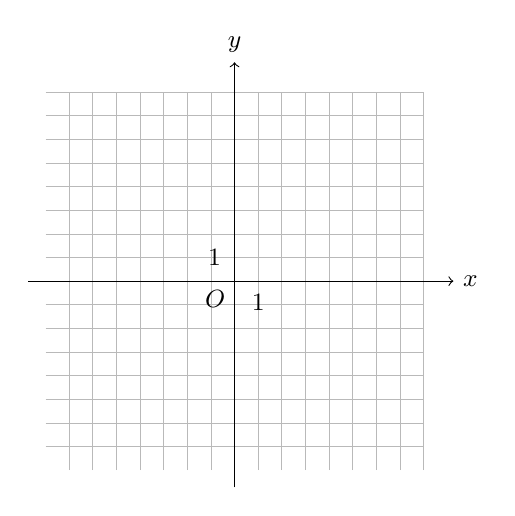
\begin{tikzpicture}[font=\small,line width=0.4pt]
  \def\u{0.30}
  \draw[gray!55,line width=0.25pt] (-2.4,-2.4) grid[step=\u] (2.4,2.4);
  \draw[->] (-2.62,0)--(2.78,0) node[anchor=west] {$x$};
  \draw[->] (0,-2.62)--(0,2.78) node[anchor=south] {$y$};
  \node[anchor=north east,inner sep=2pt] at (-0.04,-0.04) {$O$};
  \node[anchor=north,inner sep=3pt] at (\u,-0.06) {$1$};
  \node[anchor=east,inner sep=3pt] at (-0.06,\u) {$1$};
\end{tikzpicture}
